\documentclass{beamer}
\usepackage[utf8]{inputenc}

\usetheme{Madrid}
\usecolortheme{default}

% For Polish langage
\usepackage[T1]{fontenc}
% \usepackage[polish]{babel}

% For strikethrough text
\usepackage{ulem}

% For tables
\usepackage{multirow}
\usepackage{pdflscape}
\usepackage{colortbl}
\usepackage{tabulary}
\usepackage{etoolbox}
\usepackage{makecell}
\newcolumntype{P}[1]{>{\centering\arraybackslash}p{#1}}

% For figures
\usepackage{caption}
\usepackage{subcaption}

% For math
\usepackage{amsmath,amsfonts}

% For inline code listings
\usepackage{listings}
\usepackage{xparse}
\usepackage{xcolor}
\lstdefinestyle{py}{
  language=Python,
  basicstyle=\small\ttfamily,
  commentstyle=\color{green!40!black},
  keywordstyle=\color{blue},
  numberstyle=\tiny\color{gray},
  numbers=left,
  numbersep=5pt,
  backgroundcolor=\color{white},
  showspaces=false,
  showstringspaces=false,
  frame=single,
  rulecolor=\color{black},
  tabsize=4,
  captionpos=b,
  breaklines=true,
  breakatwhitespace=true,
  title=\lstname,
  caption=\lstname
}

% For algorithms
\usepackage{algorithm,algpseudocode}


% Arrows
\usepackage{tikz}
\usetikzlibrary{shapes.arrows}
\tikzset{
    myarrow/.style={
        draw,
        fill=orange,
        single arrow,
        minimum height=5ex,
        single arrow head extend=1ex
    }
}
\newcommand{\arrowup}{\tikz [baseline=-0.5ex]{\node [myarrow,rotate=90] {};}}
\newcommand{\arrowdown}{\tikz [baseline=-1ex]{\node [myarrow,rotate=-90] {};}}

% Title page
\title[WAW 2024]{19th Workshop on Modelling and Mining Networks}
\subtitle{Network Diffusion --- Framework to Simulate Spreading Processes in Complex Networks}
\author[Micha{\l} Czuba et al.]{
    \textbf{Micha{\l} Czuba} \inst{1},
    Mateusz Nurek \inst{1},
    Damian Serwata \inst{1},
    Yu-Xuan Qi \inst{2},
    Mingshan Jia \inst{2},
    Katarzyna Musial \inst{2},
    Rados{\l}aw Michalski \inst{1},
    Piotr Br{\'o}dka \inst{1}
}
\institute[]{
  \inst{1} Wroc{\l}aw University of Science and Technology\\
  \inst{2} University of Technology Sydney
}
\date[05.06.2024]{05.06.2024}
\logo{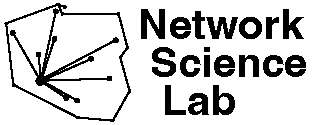
\includegraphics[height=0.5cm]{figures/nsl.pdf}}

% What will be displayed at the beginning of each section and at the end of document
% \AtBeginSection[]
% {
%   \begin{frame}
%     \begin{center}
%         \huge \secname
%     \end{center}
%   \end{frame}
% }
\AtEndDocument{
    \addtocounter{framenumber}{-1}
    \begin{frame}[c]
        \begin{center}
            \huge Thank you for your attention!
        \end{center}
        \begin{figure}
            \centering
            
\includegraphics[width=5cm]{figures/qr_code.png}
        \end{figure}
    \end{frame}
}

\begin{document}

\frame{\titlepage}

\begin{frame}{Agenda}
    In this talk, I will introduce a computational library --- \lstinline[style=py]{network-diffusion}. 
    Here is the agenda:
    \tableofcontents
\end{frame}

\section{Motivation}

\begin{frame}{\secname}
    Spreading phenomena are one of the issues considered by a network science. They can be obeserved
    in various areas like: dynamics of political opinions, marketing campaigns, spread of epidemics,
    computer viruses, etc.
    \begin{figure}
        \centering
        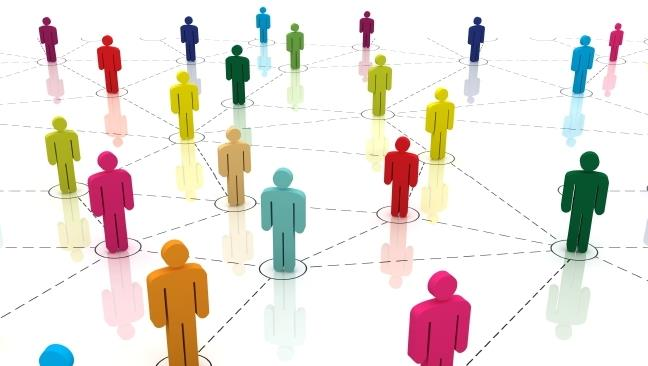
\includegraphics[width=.7\textwidth]{figures/social_network.jpg}
        \caption{Artistic representation of a social network.\footnote{Source: \url{
        www.uniroma3.it/articoli/seminario-biased-opinion-dynamics-when-the-devil-is-in-the-details-138122}
        }}
    \end{figure}
\end{frame}

\begin{frame}{\secname}
    Analytical approaches are often insufficient for large graphs, prompting researchers to use 
    computational methods, i.e. simulations.

    \begin{center}
        \vspace{1em}
        \arrowdown
        \vspace{1em}
    \end{center}
    
    Thus, like in other branches of computer science, there have been developed tools which addres 
    that issue, allowing to avoid starting from scratch and enhancing the reproducibility
    of results.\footnote{Although network science still ingloriously stands out in this matter.}
\end{frame}

\begin{frame}{\secname}
    \begin{columns}[T]
        \begin{column}{.3\textwidth}
            Indeed, there is a bunch of tools that helps in sumulating diffusion processes in networks:
            \begin{itemize}
                \item \textbf{NDlib}\cite{ndlib},
                \item GLEaMviz\cite{gleam},
                \item SimInf\cite{siminf},
                \item STEM\cite{stem},
                \item EpiModel\cite{jenness2018epimodel},
                \item Sispread\cite{sispread},
                \item ...
            \end{itemize}
        \end{column}
        \hfill
        \begin{column}{.7\textwidth}
            \begin{figure}[ht]
                \centering
                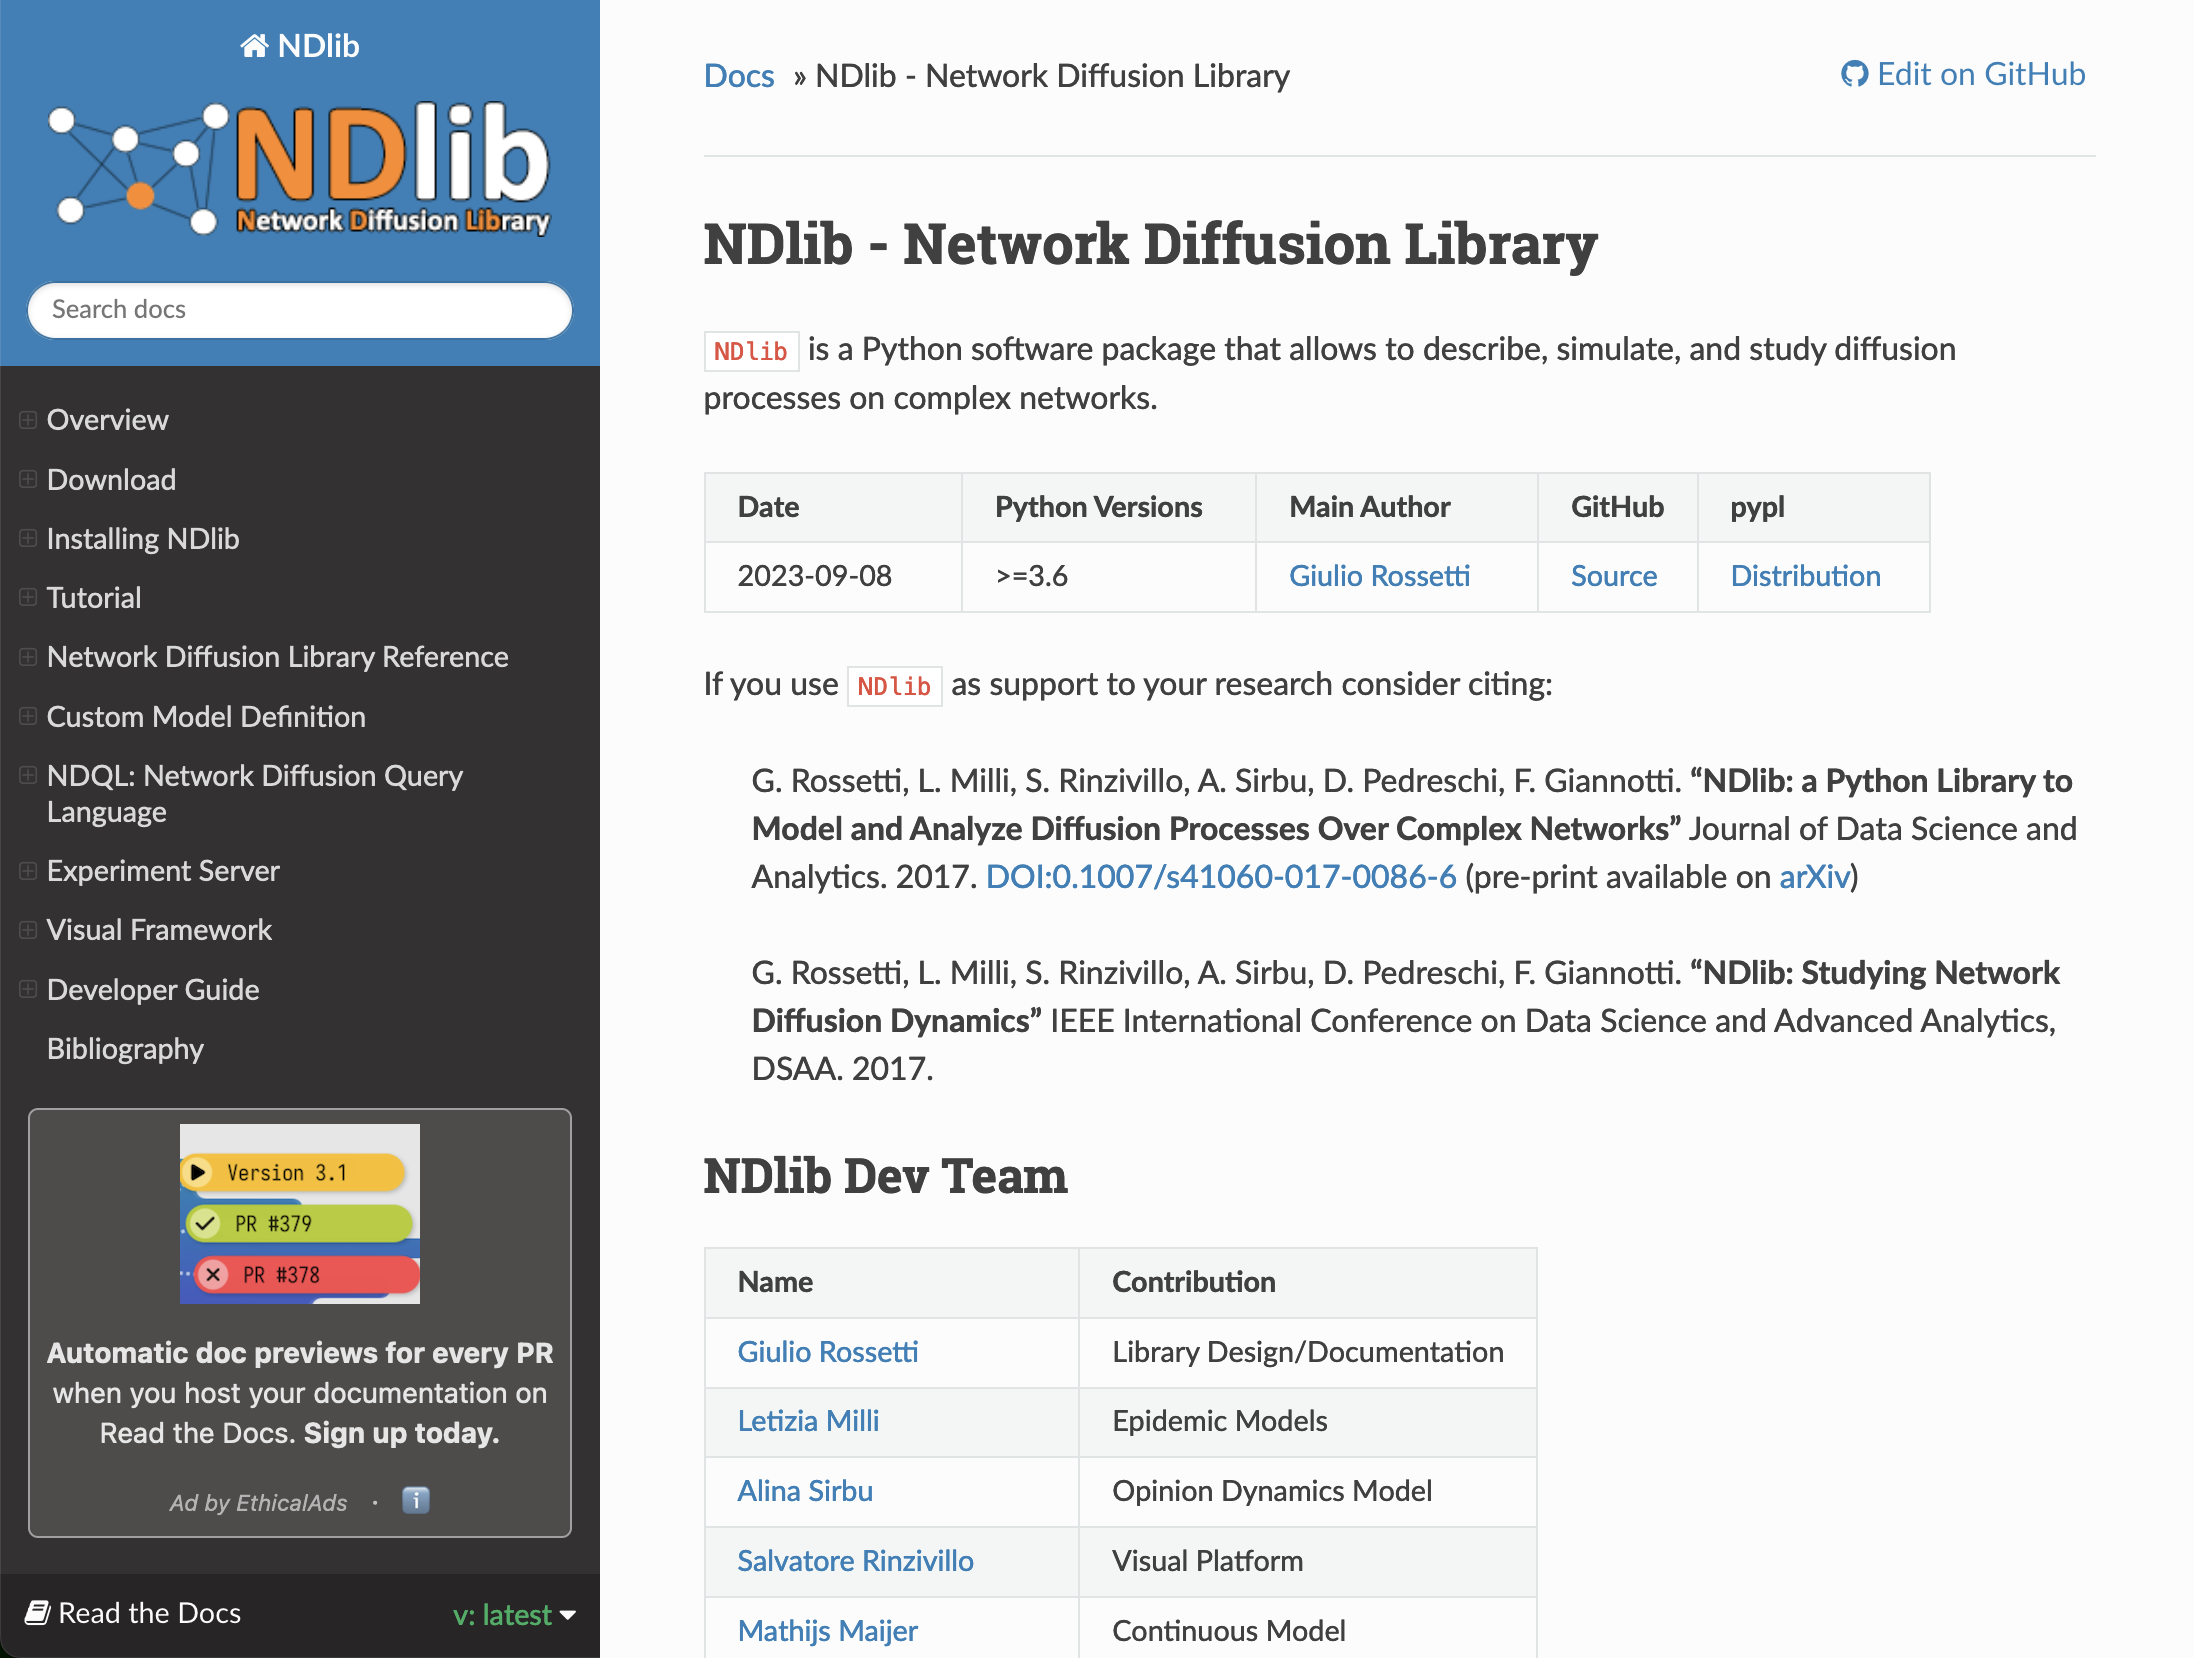
\includegraphics[width=1\textwidth]{figures/ndlib.png}
                \caption{NDlib's website.}
            \end{figure}
        \end{column}
    \end{columns}
\end{frame}

\begin{frame}{\secname}
    However, if we consider...\\
    \vspace{1em}
    \hspace{3em}...more complex network models... \\
    \vspace{1em}
    \hspace{3em}...spreading multiple processes at the same time... \\
    \vspace{1em}
    \hspace{10em}...\textbf{a gap among the available toolkits} emerges.
\end{frame}

\begin{frame}{\secname}
    A focus of our research group is oriented i.a. to: multilayer networks,
    temporal networks, spreading phenomena, data streams.
    \begin{center}
        \arrowdown
    \end{center}
    As a result of our recent activities, we decided to merge and wrap up a code we developed
    into a reusable library. We also decided to to share it with the community in an attempt of
    filling the gap in.
    \begin{center}
        \arrowdown
    \end{center}
    The main operating principles that we determined were:
    \begin{enumerate}
        \item compatibility with other tools commonly used in data science,
        \item development of a tool as a framework with open interfaces,
        \item supporting both multilayer and temporal networks,
        \item supporting spreading models with discrete states.
    \end{enumerate}
\end{frame}

\section{Key features}

\begin{frame}{\secname}
    Functionalities of \lstinline[style=py]{network-diffusion}:
    \vspace{1em}
    \begin{itemize}
        \item end-to-end simulation workflow,
        \item predefined spreading models,
        \item an interface for implementing custom spreading models,
        \item support for the temporal network models (CogSNet + discrete windows),
        \item support for the multilayer networks,
        \item centrality measures for multilayer networks.
    \end{itemize}
\end{frame}

\begin{frame}{\secname}
    Environmental requirements for \lstinline[style=py]{network-diffusion}:
    \vspace{1em}
    \begin{itemize}
        \item support for Linux, macOS, and Windows\footnote{Although we develop and use it mostly on Unix OSs},
        \item Python (preferred 3.10) compatibility,
        \item C snippets in the CogSNet module to speed-up computations,
        \item NetworkX compatibility.
    \end{itemize}
\end{frame}

\begin{frame}[fragile]{\secname}
    To prepare the experiment we have to provide a network, a spreading model and auxiliary parameters.
    Then, the simulation unfolds as follows:
    \begin{algorithmic}[1]
        \Procedure{\lstinline[style=py]{perform_propagation}}{\lstinline[style=py]{network, model, epochs}}
        \State \lstinline[style=py]{states_0} $\gets$ \lstinline[style=py]{model.determine_initial_states()}
        \State \lstinline[style=py]{model.update_network(states_0)} % \Comment{Predefined function in the \texttt{BaseModel} class}
        \For{\lstinline[style=py]{e} in \lstinline[style=py]{[1, ..., epochs]}}
        \State \quad \quad \lstinline[style=py]{states_e} $\gets$ \lstinline[style=py]{model.network_evaluation_step(network)}
        \State \quad \quad \lstinline[style=py]{model.update_network(network, states_e)}
        \EndFor
        \State \lstinline[style=py]{logs} $\gets$ generate logs from experiment \\
        \Return \lstinline[style=py]{logs}
        \EndProcedure
    \end{algorithmic}
\end{frame}

\section{Example I}

\begin{frame}{\secname}
    A story...
\end{frame}

\begin{frame}{\secname}
    \begin{center}
        \large Let's model this problem with \lstinline[style=py]{network-diffusion}!
    \end{center}
\end{frame}

\section{Example II}

\begin{frame}{\secname}
    A story...
\end{frame}

\begin{frame}{\secname}
    \begin{center}
        \large Let's model this problem with \lstinline[style=py]{network-diffusion}!
    \end{center}
\end{frame}

\section{Resources and references}

\begin{frame}[fragile]{\secname}
    The library can be installed via:
    \begin{center}
        \large
        \begin{verbatim}
            pip install network-diffusion
        \end{verbatim}
    \end{center}
    Other useful resources have also been published:
    \begin{itemize}
        \item PyPI website: \url{pypi.org/project/network-diffusion}
        \item GitHub page: \url{github.com/anty-filidor/network_diffusion}
        \item Reference guide: \url{network-diffusion.readthedocs.io}
        \item A preprint of the paper: \url{arxiv.org/abs/2405.18085}
    \end{itemize}
\end{frame}



% \begin{frame}{\subsecname}
%     Contribution -- we conducted a study on the disease-awareness model (SIR-UA)
%     to assess the effectiveness of measures against the spread of COVID-19:
%     \textcolor{red}{lockdown}, \textcolor{red}{wearing masks}, or \textcolor{red}{no restrictions}
%     based on real parameters published in medical scientific literature (e.g., Lancet):
%     \begin{columns}[T]
%         \captionsetup{font=scriptsize}
%         \begin{column}{.5\textwidth}
%             \begin{table}
%             \centering
%             \caption{Transition weights with explanation.}
%             \resizebox{1\textwidth}{!}{%
%             \begin{tabular}{c|c|p{4cm}}
%             Symbol & Formula / Value & Description \\ \hline
%             $\alpha$ & $0.19$ & probability of infection for unaware agents \\ \hline
%             $\alpha'$ & \makecell{
%                 $\lambda\alpha;$ \\ \textcolor{red}{$\pmb{\lambda \in \{ 0.1, 0.35, 1\}}$}
%             } & probability of infection for aware agents \\ \hline
%             $\beta$ & $0.10$ & probability of recovery \\ \hline
%             $\gamma$ & $0.01$ & probability of awareness for uninfected agents \\ \hline
%             $\delta$& $\gamma + 1 - 0.3$ & probability of awareness for infected agents \\ \hline
%             \end{tabular}%
%             }
%             \end{table}
%         \end{column}
%         \begin{column}{0.5\textwidth}
%         \begin{figure}
%             \centering
%             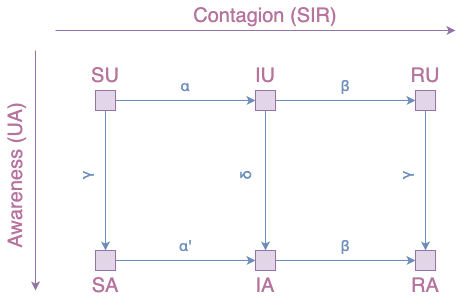
\includegraphics[width=\textwidth]{figures/sir_ua/sir_ua.png}
%             \caption{State and transition graph for SIR-UA.}
%         \end{figure}
%         \end{column}
%       \end{columns}
% \end{frame}

% \begin{frame}{\subsecname}
%     Conclusions -- for each of the investigated networks (ER, SF, real), 
%     sanitary restrictions have an impact on the peak number of infections, which
%     is of significant importance in the context of healthcare system capacity
%     during epidemics.
%     \begin{figure}[ht]
%         \centering
%         % \includegraphics[width=.8\textwidth]{figures/sir_ua/sir_ua_aucs.png}
%         % \includegraphics[width=.8\textwidth]{figures/sir_ua/sir_ua_sf.png}
%         \includegraphics[width=.8\textwidth]{figures/sir_ua/sir_ua_er.png}
%         \caption{Infection (L) and awareness (R) curves for ER network.}
%     \end{figure}
% \end{frame}


% \subsubsection{Influence Maximisation Problem}

% \begin{frame}{\subsubsecname}
%     \begin{figure}
%         \centering
%         \includegraphics[width=.7\textwidth]{figures/im_framework.pdf}
%         \caption{Components needed to define the influence maximisation problem.}
%     \end{figure}
% \end{frame}

% \begin{frame}{\subsubsecname}
%     We can distinguish three groups of methods for selecting seed set (i.e. 
%     ininitally active agenst "patients zero"):
%     \begin{itemize}
%         \item simulation-based
%         \begin{itemize}
%             \item ...
%         \end{itemize}
%         \item heuristic-based
%         \begin{itemize}
%             \item \textbf{rank refinement}
%             \item model reduction
%         \end{itemize}
%         \item mixed approaches
%         \begin{itemize}
%             \item ...
%         \end{itemize}
%     \end{itemize}
%     Methods from the rank-refining subgroup are based on creating ranked lists of
%     agents, without the need for information about the spreading model.
% \end{frame}

% \begin{frame}{\subsubsecname}
%     Constraints can be imposed on the problem of selecting seeds. This
%     could be a budget constraint, i.e., we can use only $s$ agents as a seed set
%     (the smaller the budget, the harder it gets to cover entire network by the
%     process).
% \end{frame}

% \subsubsection{Spreading Model}
% \begin{frame}{\subsubsecname}
%     How does the spreading model work?
%     \begin{itemize}
%         \item an environment --- a network model (i.e. temporal, static, directed etc.),
%         \item defined states of agents (usually: active / inactive),
%         \item defined a function determining when an agent changes state (usually
%         based on an external impulse from its neighbours),
%     \end{itemize}
%     In the literature, the most commonly considered spreading models are: the 
%     Independent Cascade Model and the \textbf{Linear Threshold Model}. \\
%     Multilayer networks, the issue is determining who is the subject of
%     diffusion: node or actor (there are many ambiguities in the literature
%     w.r.t. this problem; we used the latter approach).
% \end{frame}

\begin{frame}[allowframebreaks]
    \frametitle{\secname}
    \bibliographystyle{amsalpha}
    \bibliography{references.bib}
\end{frame}

\addtocounter{framenumber}{1}

\end{document}


% nawiązać do pracki damianac